\subsection{Bedienung des Editors}
Der Editor ist über den Text, Draw, Shape oder Image Button erreichbar. Genau wie im Reader erscheint ein Button Choose file. Je nachdem ob man auf Text, Draw, Shape oder Image geklickt hat, wird als erstes der Text-, Zeichen-, Geometrie- oder Bildeditor geöffnet.

\subsection{Textbearbeitung}
Hat man den Texteditor aufgerufen, so präsentiert sich einem der Editor in folgenden Abbildungen \ref{fig:texteditor} und \ref{fig:texteditor2}.

\begin{figure}[!htbp]
	\centering
	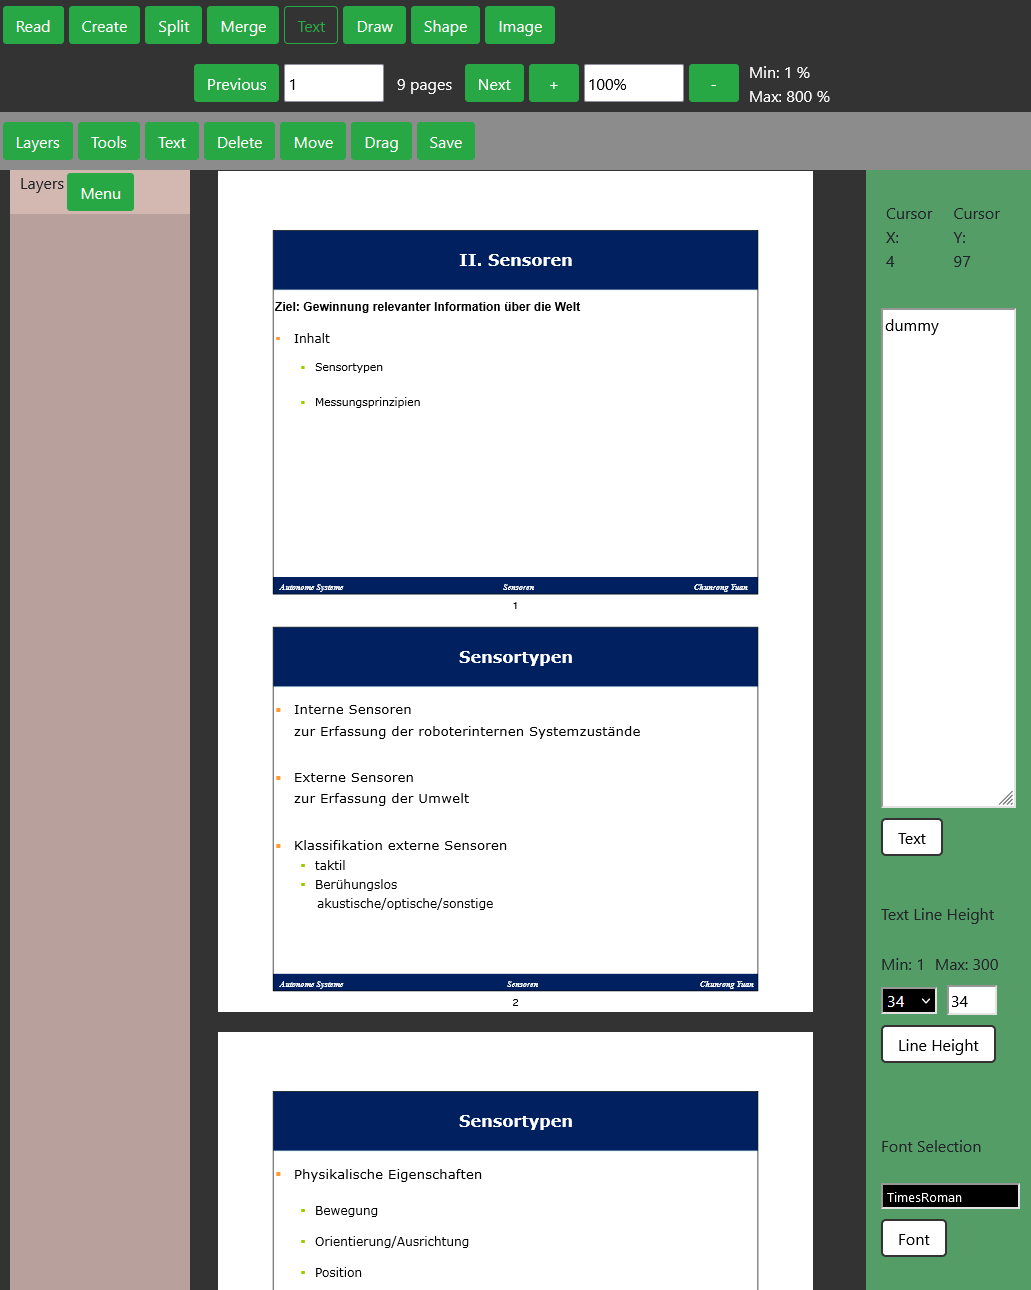
\includegraphics[width=1\textwidth]{"images/texteditor.png"}
	\caption{Startseite des Texteditors der PDF Web App}
	\label{fig:texteditor}
\end{figure}

\begin{figure}[!htbp]
	\centering
	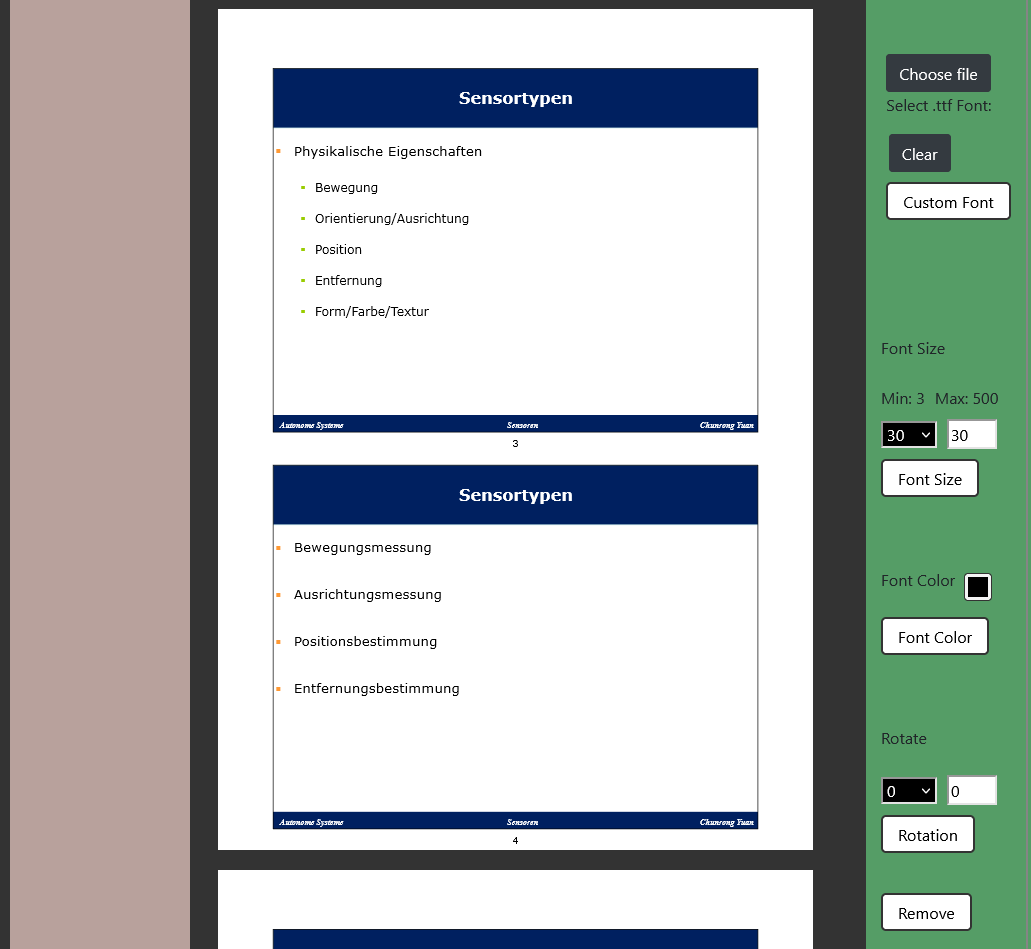
\includegraphics[width=1\textwidth]{"images/texteditor2.png"}
	\caption{Mehr Tools der Startseite des Texteditors der PDF Web App}
	\label{fig:texteditor2}
\end{figure}

Mit dem Button Text in der grauen Leiste und nachfolgendem Klick aufs geöffnete Dokument kann man einen Text hinzufügen mit dem Platzhaltertext dummy. Unter dem Text erscheint eine dunkelrote control box, auf die man alle Operationen in Tools im Box Mode anwenden kann. Der Box Mode ist standardmäßig eingestellt. Alle Operationen im rechten Tools Seitenmenü beziehen sich jeweils auf das aktuelle Editor Element und sind nur auf diesem anwendbar. Ich werde zunächst alle Operationen im Box Mode beschreiben und später auf den Layer Mode eingehen. Man kann mehrere Texte ohne erneut Text drücken zu müssen dem PDF Dokument hinzufügen. Mit dem Delete Button und nachfolgendem Klick in eine oder mehrere control boxen im Box Mode können Texte wieder gelöscht werden. Move verschiebt einzelne Texte durch mit der Maus gedrückte control box. Wenn die Maus losgelassen, nachdem die control box verschoben wurde, springt der Text an die verschobene Stelle. Ganz oben im grünen Tools Seitenmenü werden dem Betrachter die x- und y-Koordinaten der Maus auf der PDF Seite angezeigt, wenn die Maus über eine Seite bewegt wird. Darunter kann man in der textarea den Text editieren. Es werden auch Zeilenumbrüche berücksichtigt. Nachdem man den dummy Text überschrieben hat, einem Klick auf den weißen Text Button und ein oder mehrere Klicks in control boxen, kann der Text angewendet werden. Alle Operationen in Tools werden genau gleich ausgeführt: Man tätigt seine Einstellung, drückt mit der linken Maustaste auf den weißen Button für die jeweilige Operation und klickt daraufhin auf ein oder mehrere Textelemente nacheinander. Darunter kann man den Zeilenabstand einstellen. Entweder verwendet man das selection menu mit voreingestellten Werten oder man gibt einen gewünschten Wert manuell in das input field ein. Alle selection menus und input fields in jedem Editor zeigen die default Werte, mit denen ein neu hinzugefügtes Element konfiguriert ist, an. Falls man zuletzt das selection menu betätigt hat, überschreibt es den Wert im input field und umgekehrt. Maßgeblich ist, was man zuletzt betätigt hatte. Dieses Verhalten habe ich bei jeder selection menu und input field Kombination programmiert. Einen benutzerdefinierten Font kann man durch den dunkelgrauen Choose file Button auswählen und er erscheint in der Liste. Der zuletzt hochgeladene Font wird ausgewählt. Mittels clear kann man einen ausgewählten Font aus der Liste entfernen, was nicht heißt, dass er auch auf dem angewendeten Text entfernt wird. Die Fontgröße kann man ebenfalls wie die Zeilenhöhe mit selection menu und input field justieren. Bei der Fontfarbe klickt man auf das initial schwarze Quadrat, was die aktuelle Farbe zeigt, und es öffnet sich ein color picker Menü. Hier kann man die Farbe und Transparenz einstellen. Die Werte kann man sich in RGBA, HSLA oder HEX formatieren lassen. Mit Klick auf die beiden kleinen senkrechten Pfeile im color picker wird jeweils das Format gewechselt. Die Abbildung \ref{fig:texteditor3} zeigt einen modifizierten Text mit benutzerdefiniertem Font und Abbildung \ref{fig:fontcolor} zeigt den color picker für die Fontfarbe. 

\begin{figure}[!htbp]
	\centering
	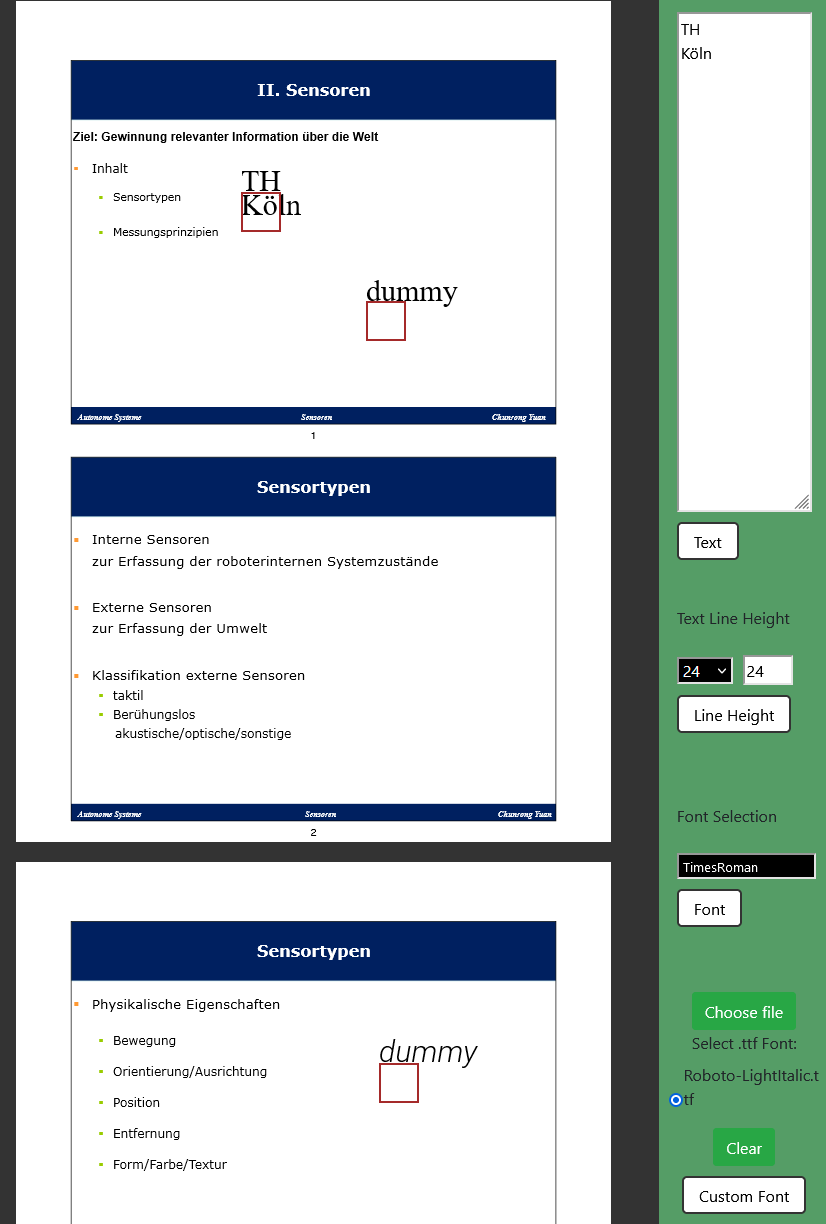
\includegraphics[width=1\textwidth]{"images/texteditor3.png"}
	\caption{Modifizierter Text im Texteditor der PDF Web App}
	\label{fig:texteditor3}
\end{figure}

\begin{figure}[!htbp]
	\centering
	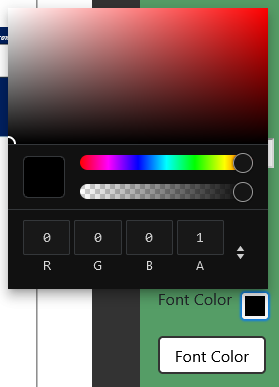
\includegraphics[width=0.6\textwidth]{"images/fontcolor.png"}
	\caption{Color picker für die Fontfarbe des Texteditors der PDF Web App}
	\label{fig:fontcolor}
\end{figure}

Als vorletzte Option kann man den Text absolut drehen. In der Praxis bedeutet das, dass immer eine Benutzereingabe für Rotation das Element mit 0 Grad Rotation auf den gewünschten Wert rotiert. Folglich passiert keine Veränderung, wenn man den gleichen Rotationswert 2 Mal hintereinander ausführt. Abschließend können alle Textelemente im Dokument mit dem Remove Button auf einen Schlag gelöscht werden. 